\documentclass[a4paper,12pt]{article}
%\usepackage[catalan]{babel}
\usepackage[utf8]{inputenc}
\usepackage{amsfonts}
\usepackage[colorlinks=true]{hyperref}
\usepackage[left=3cm,right=3cm]{geometry}
\usepackage{graphicx}
\usepackage{url}
\usepackage{subfigure}

\title{The Sphere of the Earth \\ Description and Technical Manual \\ {\small December 20, 2012 } }
\author{Daniel Ramos \footnote{E-mail: \texttt{daniel.ramos@mmaca.cat}}\\MMACA (Museu de Matemàtiques de Catalunya)}

\date{}

\begin{document}
\maketitle

\section{The exhibit}

The exhibit we are presenting explores the science of cartography and the geometry of the sphere. Althoug this subject has been widely treated on science exhibitions and fairs, our proposal aims to be a more comprehensive and complete treatment on the subject, as well as to be a fully open source, documented material that both museographers and public can experience, learn and modify.

The key concept comes from the problem of representing the spherical surface of the Earth onto a flat map. Studying this problem is the subject of cartography, and has been an important mathematical problem in History (navigation, position, frontiers, land ownership...). An essential theorem in Geometry (Gauss' Egregium theorem) ensures that there is no perfect map, that is, there is no way of representing the Earth keeping distances at scale. However, this is exactly what makes cartography a discipline: developing several different maps that try to solve well enough the problem of representing the Earth.

A common activity is comparing an Earth globe with a (Mercator) map, observing that distances are not preserved. Our module explores far beyond that. We present:
\begin{itemize}
 \item Several different maps, currently 6 map projections are used, each one featuring different special properties. Printed at nominal scale 1:1 of a model globe.
 \item \emph{The script programs} that generate these pictures. Generating a map takes less than 50 lines of code, anyone could generate his own.
 \item A collection of tools and models: a flexible ruler to be used over the globe, plane and spherical protractors, models showing longitude and latitude... To be used on several activities.
 \item \emph{A computer program} that shows the Tissot's indicatrix for the maps. This is a valuable tool for seeing how much a map distorts the Earth.
\end{itemize}

Our main contribution is clearly the software we developed. However, the module we present is both physical and virtual, since the
interaction the sphere, the scaled maps and the simulation software is much richer than seeing only the maps and simulations on a screen.

The didactical potential of this module is wide. Lots of contents can be linked with this module, including: basic Geometry and
trigonometry on the sphere, applicatinos and transformations, Cartography, Geography and sociocultural regions, History of the discoveries,
advanced Differential geometry, Non-euclidean geometries, Computer programming, etc. Cultural contents are very interesting in seeking a
big scope. Public can find subject appearingly non-mathematic, such as History, being higly influenced by the mathematical laws governing
the world and the knowledge that mankind had of them at each time.


\section{Parts of the exhibit}
The inventory of the parts of our exhibit is the following:
\begin{itemize}
 \item A globe at 20 cm diameter, thus at scale 1:63,710,000 of the Earth.
 \item A collection of 6 maps, at nominal scale 1:1 of the globe.
 \item A flexible ruler (tape measure) with scale in km and in degrees for the globe.
 \item A transparent hemispherical model for the longitude and latitude.
 \item A plane and a spherical protractors.
 \item A collection of plane solid foam pieces with she shape of the continents on some equal-area projections.
 \item A collection of spherical shell pieces with the shape of the continents.
 \item A computer running the program ``The Sphere of the Earth''.
\end{itemize}

Some comments about each component:

\subsection{Globe}
A globe of the Earth. We use a 20 cm diameter globe, this is, at scale 1:63,710,000 of the Earth. The size is important because all maps
must be done at nominal scale 1:1 to this globe. For instance, in a Mercator projection the equator is shown at true scale, therefore the
width of the poster of the Meractor map must equal the length of the equator of the globe (namely $2\pi\cdot 10 \mathrm{cm} =
62.8\mathrm{cm}$). This size makes the posters small enough as to be printed on a DIN-A0 sheet, available at most reprographics. It is also
a convenient size for a portable exhibition. A bigger size would show better on wide spaces, but it would be less portable and more
expensive to print the posters (need an industrial printer).

We bought a Stellanova globe, model 892094\footnote{\url{http://www.stellanova-europe.com/fileadmin/stv_dateien/datasheets/892094.pdf}},
because it is magnetic and can be easily detached from its support. It would be nicer to have the same picture on the globe and on the maps,
but this would be undoubtelly more expensive and difficult to achieve than just buying one.

\subsection{Maps}
A map projection is just a mathematical formula that sends any point on the Earth (longitude and latitude) to a point on the plane ($x,y$
coordinates). We implemented these formulae in a small script program, and we are able to generate any map. The source geographical data
comes from a bitmap image derivated from NASA satellite imagery\footnote{\url{http://visibleearth.nasa.gov/view.php?id=57752}} This has the
highest quality and is on the public domain thanks to NASA's policy. 

Maps are provided at nominal scale 1:1 of the globe. This means that points shown at true scale (such as the equator in Mercator projection) have the same size as the corresponding points on the sphere. Also, area-preserving maps have the same area as the globe (namely $4\pi\cdot (10\mathrm{cm})^2 = 1256.6 \mathrm{cm}^2$). This makes easier to see which parts of the map are shrinked or expanded. 

We provide the images, but more important, we provide the code to generate them, so anyone can modify the maps. For instance, some of the maps are azimuthal or oblique, meaning that some point has been chosen to be at the center of the map. We chose Barcelona because it is the main city in our region, but any location could be used just changing the program parameters. There is, of course, some professional software that also does the job, but our small program encourages people to look at the 50 lines of code and understand the maths and algorithms behind. On that side, this module does not only uses open source programs, but also teaches and encourages the open source philosophy. We think this could be a good example project for introducing people to programming.

\subsection{Tools}
A good collection of materials for spherical geometry is the kit ``Lénárt Sphere''\footnote{\url{www.lenartsphere.com}} , that contains
spherical shells (also $20\mathrm{cm}$ diameter) and a spherical protractor. 

We use a flexible ruler, printed over a strip of polyester canvas (see the attached pdf file), with a double scale, both in degrees and in
kilometers. The equivalence 40,000 km = 360º holds on the Earth along any great circle. The length of the ruler measures these 40,000 km or
360º in the 628.32 mm of the equatorial length of the globe. 

We only use units in SI, not imperial units. The original definition of meter is actually $\frac{1}{40,000,000}$ of the circumference of
the Earth (measured over a meridian).

\subsection{Models and jigsaws}
A transparent hemisphere marked with a meridian and a parallel, and apropriate markings for angles, serves as an inmediate way for defining
latitude and longitude to anyone. 

The profiles of the continents on the globe are cut on a spherical shell, and the same profiles on two equal-area projections are cut on
foam plastic sheets. This serves to make comparisons on three equal area representations of the same continent.


\section{The image scripts}
The image scripts are the programs that generate the maps for the posters. These scripts are written in Python, and need a Python
interpreter to be executed (see technical requirements in section below). These scripts are not primarily intended to be used by the public,
but for the exhibition organizer. These scripts allow customization such as modifying the scale if we intend to use a bigger globe, or
changing the center of the projection on some azimuthal and oblique maps (we chose Barcelona as the center on a cuuple of maps).

Besides the organizers, these scripts can and should be publicly available on the web for anyone. Interested visitors could download these
scripts at home after having seen the exhibition, so they could play and modify the scripts. To encourage this, however, a carefull
revision of the code and some tutorials should be done before. Anyway, this can be a very educational programming lesson.

Currently all parameters are hard-coded into the source. Input is a modified version of NASA's ``blue marble`` satellite imagery. We used a
good enough resolution for our size, but ultra-high resolution versions can be also downloaded. Output is a pdf file, since it keeps the
actual size infrmation and it is the preferred format at most reprographics. Mathematical formulae for the projections are not implemented
by us, instead we use the open source library Proj.4\footnote{\url{http://trac.osgeo.org/proj/}}.

These scripts may seem a technical part of the module, but it is the difference between providing fish and providing a fishing rod.


\section{The program}
The program named ``The Sphere of the Earth. Version 1.0.0'' is a graphical program that displays several map projections and their
Tissot's indicatrix. As explained in the Activities documentation, Tissot's indicatrix is a tool for visualizing the distortion of a map.
For a given point, a small geographic circle is depicted around it, not as a circle, but as an ellipse due to map distortion. Size,
orientation and flattening of this ellipse illustrates the distortion of the map at this point.

It is common to see diagrams with Tissot ellipses on books, atlases and Wikipedia pages about map projections. Our program draws
interactivelly this ellipses, instead of just a static image. Available software for computing Tissot's indicatrices is, as far as we know,
restricted to professional privative software, not designed to be used as an educational or recreational tool.

\subsection{Features}
The main window displays a tab selector, each tab contains a map projection, the same projections we have on the posters. When moving
the mouse pointer over the image of the map, a Tissot ellipse is overprinted. Clicking on the map leaves an ellipse at this point. On a
side label, the geographic coordinates of the pointed location are displayed. A selector allows to choose the size of the ellipses (scale
factor), and a button clears the ellipses drawn.

Tissot's ellipses are generally drawn on red. The border turns into green if the ellipse is actually a circle (conformality) and the
interior turns into green if the area is the same as the geographic disc it represents (equal-area). See the Activities documentation.

\subsection{Technical requirements}

The program is written in Python, which is a scripting language. This means that the code is not compiled, instead the source code is
provided and another program (the Python interpreter) executes each instruction. We chose this language for ease of use and being widespread
along the scientific community.

Python programs are cross-platform, since the only requirement is a working Python interpreter together with the auxiliary libraries:
\begin{itemize}
 \item Python interpreter, v2.7 or higher.
 \item numpy. Library for Numerical computations on Python.
 \item pyproj. Library for cartographic computations on Python.
 \item PyQt. Graphical libraries for Python.
\end{itemize}

\paragraph{Install on Linux (Ubuntu).} Type on a command line:\\
\texttt{\$ sudo apt-get install python python-numpy python-pyproj python-qt4} \\
\texttt{\$ python soe.py}

\paragraph{Install on Windows.} Download and install the interpreter and the libraries from their respective websites:
\begin{itemize}
 \item \url{http://python.org/ftp/python/2.7.3/python-2.7.3.msi}
 \item \url{http://sourceforge.net/projects/numpy/files/NumPy/1.7.0b2/numpy-1.7.0b2-win32-superpack-python2.7.exe/download}
 \item \url{http://pyproj.googlecode.com/files/pyproj-1.9.2.win32-py2.7.exe}
 \item \url{http://sourceforge.net/projects/pyqt/files/PyQt4/PyQt-4.9.5/PyQt-Py2.7-x86-gpl-4.9.5-1.exe}
 \item Double click on the file soe.py , select ``Open with...'' and select the program python.exe just installed.
\end{itemize}
A more compact, single-file distribution of the program would be desirable for Windows users. Unfortunately, this is not yet available due to technical difficulties.


\section{Future development}
The exhibit we present is totally usable, but there will probably bugs and typos on the software and documentation, as well as plenty of room for improvement. Some features are being developed but are not present nowadays due to time constraints. Other features are still projects. We summarize here some of these future improvements.

\paragraph{Open software repository.} After being presented to the competition, the software will be uploaded to some open software
repository (Sourceforge, Github...). This aims to open its developement to the community. This is a museographic and educational project,
not a professional cartographic software. Focus should be put on didactics, easy of use, and easy of reading the code. 

\paragraph{Spherical triangles calculator.} This feature is quite developed, and deals with spherical triangles. These triangles are figures over the sphere surface delimited by three arcs of maximal circles (the sides) intersecting at three points (the vertices). The feature consists on a program that shows a diagram of a spherical triangle. Given any three data of the six parameters of the triangle (three sides and three angles), the other three are uniquely determined by some spherical trigonometric formulae, analogous to the pythagorean, sine and cosine theorems on the plane. In summary, this allows to solve spherical triangles. 

Spherical trigonometry has a strong connection to geodesy. Given two locations on the Earth, what is the distance between them? To answer this question, we construct a triangle with our two locations together with the North pole. This forms a triangle, from which we can know two sides and an angle from the coordinates of the two locations. Using our calculator (using spherical trigonometry) we can obtain the required distance. This is showed on our program. We include a screenshot of the developing program.

\paragraph{Create your own maps.} At the moment all images are fixed, bitmap based. This requires a few minutes to run the scripts generating the maps, and modifying them requires a previous meditation. A faster program, working on vector images and computing only profiles for the map, together with a good user interface should allow the user to ``play with the formulas'' and just see what happens with some random customization of a map. This could be lead to show for instance the theory of conformal mappings on complex variable.

\paragraph{Geodesics.} This feature should be an obvious improvement. Pick two points on the map and you get drawn the shortest path joining them. This path will not in general be a straight line, since it is an arc over the sphere projected onto a map. Maybe a different layout for the program, viewing together several maps could improve the feeling of distortion when displayed the same geodesic path on different maps.

\paragraph{Geogebra.} It has been suggested to us that the program Geogebra could do a similar task as our program or interact in interesting ways. Geogebra has announced a forthcoming support for Python scripts, so we will keep attention on it.

\paragraph{Documentation.} We propose a series of activities to be done using this materials, and we provide some background material on the subject. However, this documentation can and should be improved with the aim of being factually correct, stratified to adapt to the knowledge of each public, and at the same time simplified and made attractive and fun. We firmly believe that this same materials can be used and profited by young scholars, intermediate and university students, just adapting the focus and scope of the activities and explanations. This is documentation task.

\section{License}

The author, Daniel Ramos Guallar, and its institution, MMACA - Museu de Ma\-te\-mà\-ti\-ques de Catalunya, agree to publish the submitted
material under a Creative Commons license BY-NC-SA, and to participate on the competition ``Mathematics of Planet Earth 2013. A competition
for an open source exhibition of virtual modules''. Subsequent versions of the software might appear on public repositories of open software
under the appropriate license. All software involved on the development of this material is free open source. Images derivated from NASA
satellite imagery, avaliable at public domain.

\section{Gallery}

\begin{figure}[h]
\begin{center}
\subfigure[Plate-Carrée]{ 
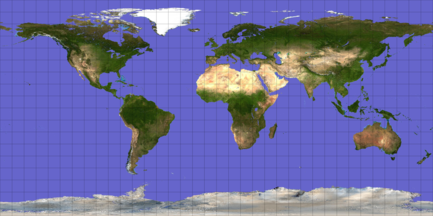
\includegraphics[scale=0.3]{platecarre_thumb.png}  }
\subfigure[Mercator]{
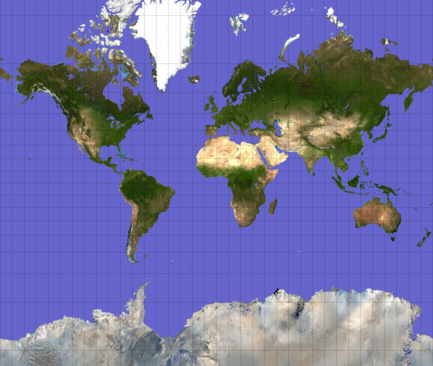
\includegraphics[scale=0.3]{mercator_thumb.png}  }

\subfigure[Gall-Peters]{
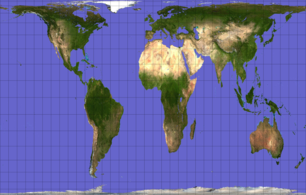
\includegraphics[scale=0.3]{gallpeters_thumb.png} }
\subfigure[Azimuthal Equidistant]{
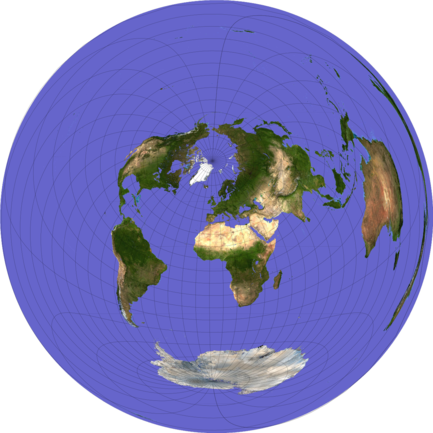
\includegraphics[scale=0.3]{aziequi_thumb.png} }

\subfigure[Gnomonic]{
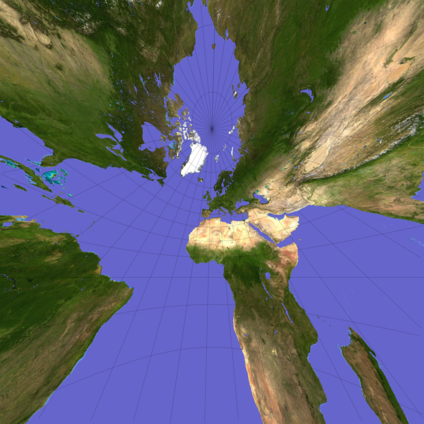
\includegraphics[scale=0.3]{gnomo_thumb.png} }
\subfigure[Mollweide]{
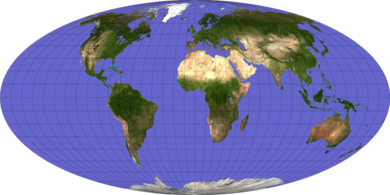
\includegraphics[scale=0.3]{mollweide_thumb.png} }

\caption{The map projections posters, shown to scale.}
\end{center}
\end{figure}
\begin{figure}[h]
\begin{center}
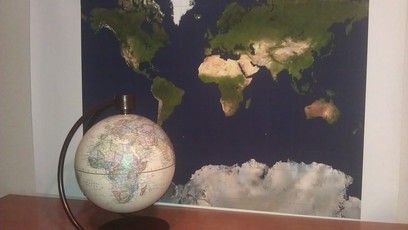
\includegraphics[width=0.6\textwidth]{globe.jpg}
\caption{The Globe.}
\end{center}
\end{figure}

\begin{figure}[h]
\begin{center}
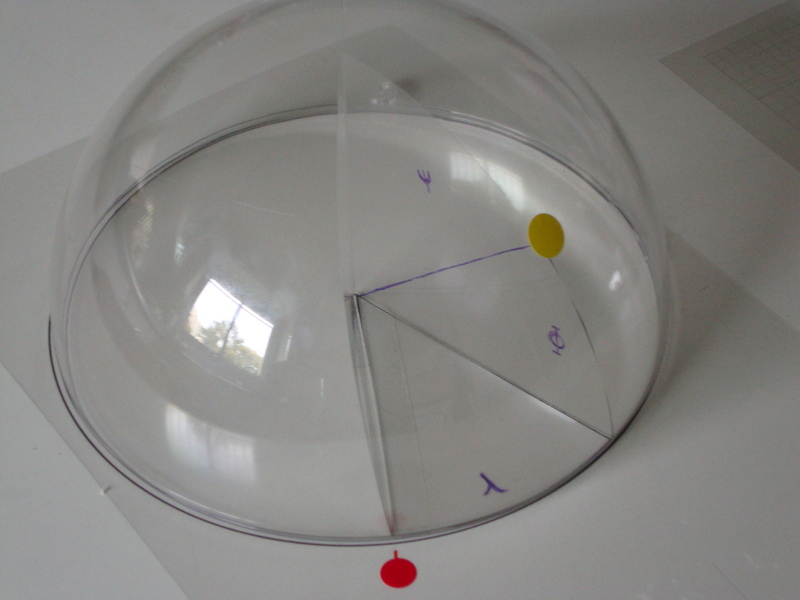
\includegraphics[width=0.6\textwidth]{latlon.jpg}
\caption{A model for longitude and latitude.}
\end{center}
\end{figure}


\begin{figure}[h]
\begin{center}

\subfigure{ 
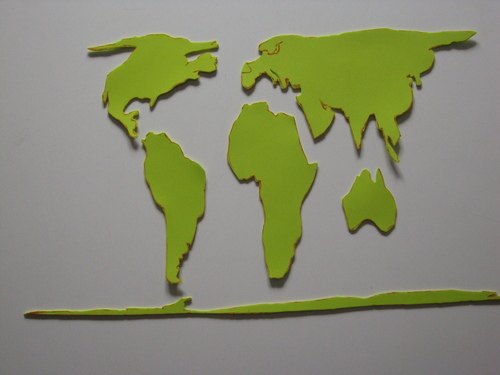
\includegraphics[scale=0.3]{peters_foamy.jpg}  }
\subfigure{
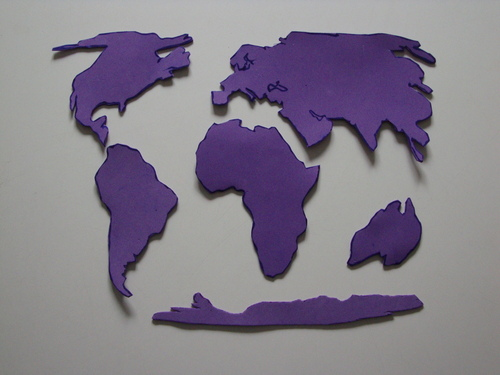
\includegraphics[scale=0.3]{mollweide_foamy.jpg}  }
\subfigure{
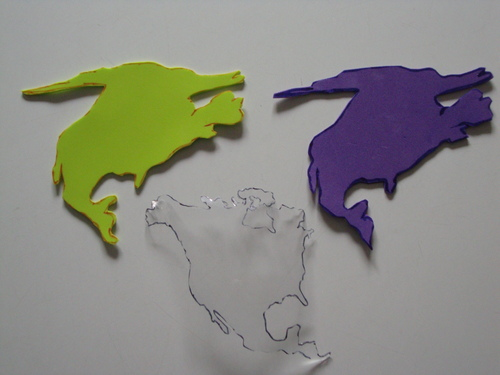
\includegraphics[scale=0.3]{profiles.jpg} }

\caption{profiles for the continents.}
\end{center}
\end{figure}


\begin{figure}[h]
\begin{center}
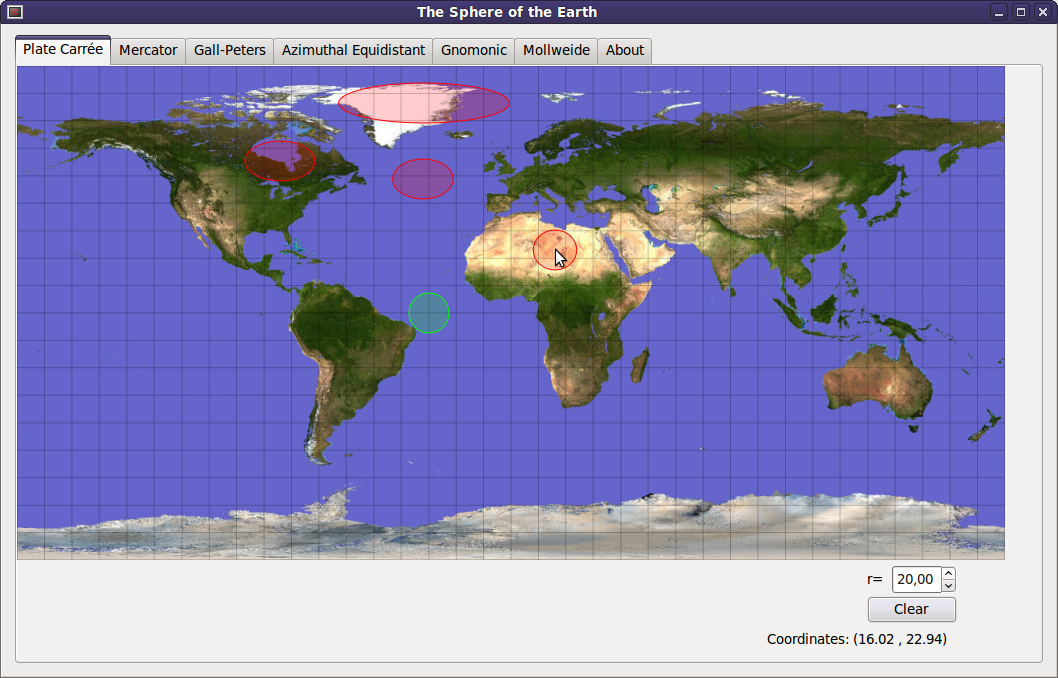
\includegraphics[width=0.8\textwidth]{soe1.png}
\caption{A screenshot of the program.}
\end{center}
\end{figure}
 
 \begin{figure}[h]
\begin{center}
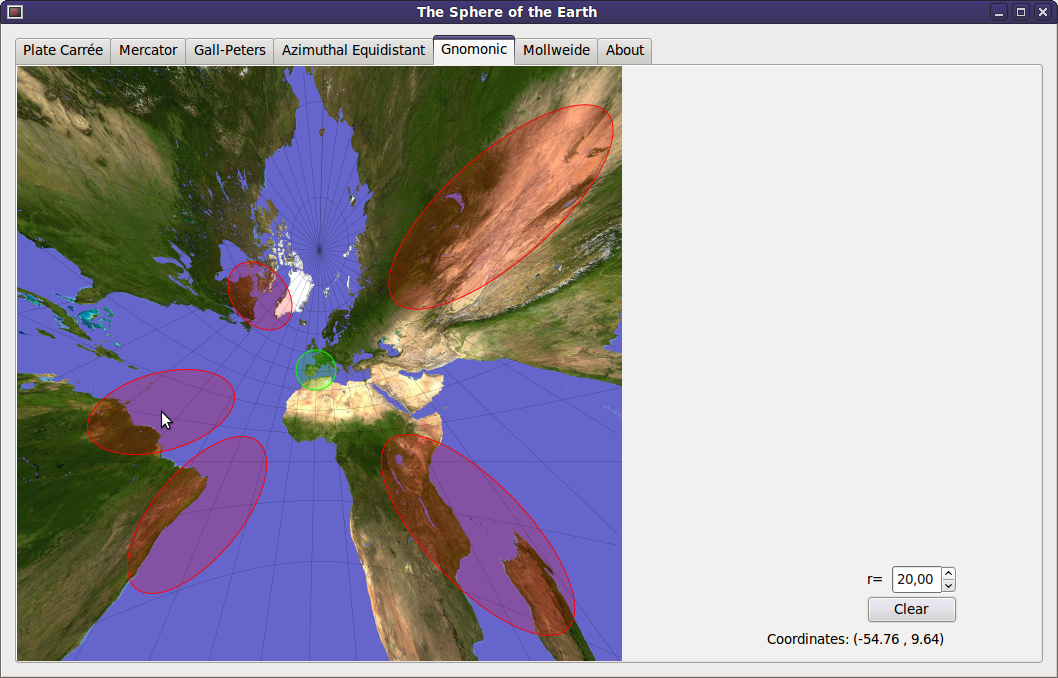
\includegraphics[width=0.8\textwidth]{soe2.png}
\caption{A screenshot of the program.}
\end{center}
\end{figure}

 
 \begin{figure}[h]
\begin{center}
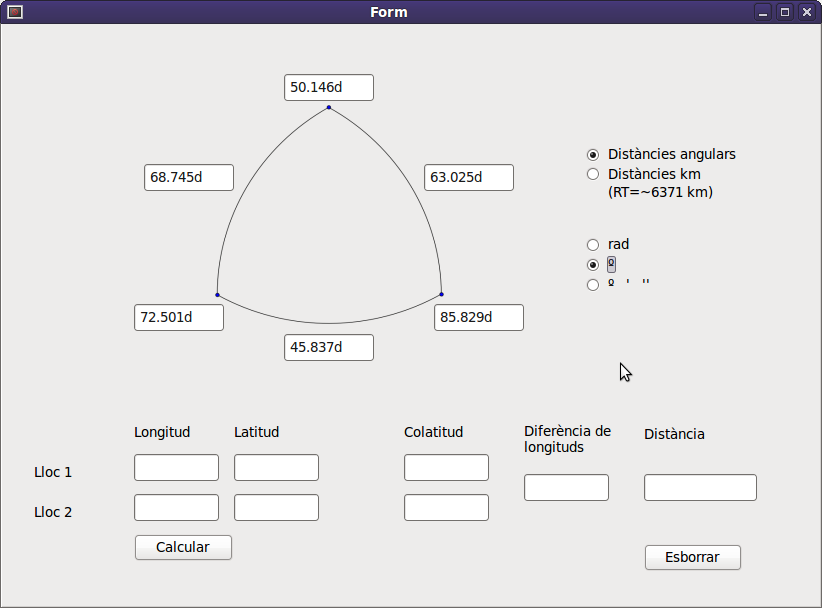
\includegraphics[width=0.8\textwidth]{triang.png}
\caption{A screenshot of the spherical triangle calculator (in developement).}
\end{center}
\end{figure}
 
 
\end{document}

